%%%%%%%%%%%%%%%%%%%%%%%%%%%%%%%%%%%%%%%%%
% OIST Doctoral Thesis - Final bound version
% LaTeX Template
% Version 0.2 (2016/04/06)
%
% This version is the final binding version which will be published.
%
% Original author:
% Jeremie Gillet
%
%%%%%%%%%%%%%%%%%%%%%%%%%%%%%%%%%%%%%%%%%

%----------------------------------------------------------------------------------------
%	PACKAGES AND OTHER DOCUMENT CONFIGURATIONS
%----------------------------------------------------------------------------------------

\documentclass[12pt]{book} % 12 pt font, two-sided book style
\usepackage[a4paper, includehead, headheight=0.6cm, inner=3cm ,outer=2.5cm, top=2.5 cm, bottom=2.5cm]{geometry}  % Changing size of document
\usepackage[english]{babel} % The document is in English
\usepackage[utf8]{inputenc} % UTF8 encoding
\usepackage[T1]{fontenc} % Font encoding

\usepackage{graphicx} % For including images
\graphicspath{{./Images/}} % Specifies the directory where pictures are stored

\usepackage{longtable} % tables that can span several pages
\usepackage[bf]{caption} % caption: FIG in bold
\usepackage{fancyhdr} % For the headers

\newcommand{\numberedchapter}{ % Preparation for numbered chapters
	\cleardoublepage % To make sure the previous headers are passed
	\fancyhead[RE]{{\bfseries \leftmark}}% Headers for left pages
	\fancyhead[LO]{{\bfseries \rightmark}}}% Headers for right pages
\newcommand{\unnumberedchapter}[1]{ % Preparation for unnumbered chapters
	\cleardoublepage % To make sure the previous headers are passed
	\addcontentsline{toc}{chapter}{#1} % Also adds the chapter name to the Contents
	\fancyhead[RE]{{\bfseries #1}} % Headers for left pages
	\fancyhead[LO]{}}%Headers for right pages

\usepackage{emptypage} % No headers on an empty page

\usepackage{eso-pic} % For the background picture on the title page
\newcommand\BackgroundPic{%
\put(-250,-160){%
\parbox[b][\paperheight]{\paperwidth}{%
\vfill
\centering
\includegraphics[width=\paperwidth]{symbol.jpg}%
\vfill
}}}

\usepackage{hyperref} % Adds clickable links at references

%----------------------------------------------------------------------------------------
%	ADD YOUR CUSTOM VALUES, COMMANDS AND PACKAGES
%----------------------------------------------------------------------------------------

% Open Preamble/mydefinitions.tex and enter some values (name, thesis title...) 
% and include your own custom LaTeX functions and packages

%----------------------------------------------------------------------------------------
%	VALUES FOR THE THESIS
%----------------------------------------------------------------------------------------

\newcommand{\name}{MohammadReza Ebrahimi} % Author name
\newcommand{\thesistitle}{} % Title of the thesis
\newcommand{\submissiondate}{October, 2022} % Submission date "Month, year"
\newcommand{\advisor}{Ashish Khisti} % Supervisor name


%----------------------------------------------------------------------------------------
%	BIBLIOGRAPHY STYLE (pick the style you want)
%----------------------------------------------------------------------------------------

\usepackage[square, numbers, sort&compress]{natbib} % for bibliography - Square brackets, citing references with numbers, citations sorted by appearance in the text and compressed (as in [4-7])
%\usepackage[longnamesfirst,round]{natbib} % Natural Sciences bibliography

\bibliographystyle{Preamble/physics_bibstyle} % You may use a different style adapted to your field
%\bibliographystyle{unsrtnat} % You may use a different style adapted to your field


%----------------------------------------------------------------------------------------
%	YOUR PACKAGES (be careful of package interaction)
%----------------------------------------------------------------------------------------

\usepackage{amsthm,amsmath,amssymb,amsfonts,bbm}% Math symbols


\usepackage{graphicx}
\usepackage{dsfont}
\usepackage{dirtytalk}
\usepackage{bm}
\usepackage{import}
% \usepackage{authblk}
\usepackage{caption}
\usepackage{subcaption}
% \usepackage{sectsty}% http://ctan.org/pkg/sectsty
% \sectionfont{\MakeUppercase}
% \usepackage[utf8]{inputenc} % allow utf-8 input
% \usepackage[T1]{fontenc}    % use 8-bit T1 fonts
\usepackage{hyperref}       % hyperlinks
\usepackage{url}            % simple URL typesetting
\usepackage{booktabs}       % professional-quality tables
\usepackage{algorithm2e}[ruled]
% \usepackage{nicefrac}       % compact symbols for 1/2, etc.
% \usepackage{microtype}      % microtypography
\hypersetup{colorlinks=true, linkcolor=blue, citecolor=blue, urlcolor = blue}


%----------------------------------------------------------------------------------------
%	YOUR DEFINITIONS AND COMMANDS
%----------------------------------------------------------------------------------------

% New Commands
\newcommand{\bea}{\begin{eqnarray}} % Shortcut for equation arrays
\newcommand{\eea}{\end{eqnarray}}
\newcommand{\e}[1]{\times 10^{#1}}  % Powers of 10 notation

% Defining a theorem box for Criteria
\newtheorem{critere}{Criterion}
\newcommand{\crit}[2]{
\begin{center}  
\fbox{ \begin{minipage}[c]{0.9 \textwidth}
\begin{critere}
\textbf{\textup{ #1}} --- #2
\end{critere}
\end{minipage}  } \end{center}
}

\newtheorem{theorem}{Theorem}[section]
\newtheorem{corollary}{Corollary}[theorem]
\newtheorem{lemma}[theorem]{Lemma}
\newtheorem{remark}[theorem]{Remark}
%----------------------------------------------------------------------------------------
%	YOUR DEFINITIONS AND COMMANDS
%----------------------------------------------------------------------------------------

\def\reals{\mathbb{R}} % Real number symbol
\def\W{\bm{W}}
\def\w#1{\W^{(#1)}}
\def\y{\bm{Y}}
\def\Y#1{\y^{(#1)}}
\def\X{\bm{X}}
\def\K{\bm{K}}
\def\sv#1{\rho_{(#1)}^2}
\def\rv#1{\sigma_{#1}^2}
\def\q{Q}
\def\t{T}
\def\m{M}
\def\p{P}
\def\params{\bm{\theta}}
\def\spcov#1{\bm{\Psi}^{(#1)}}
\def\A{\bm{A}} 
\def\rvs{\bm{\sigma}^2}

\def\ytrain#1{$\y^{\text{train }}_#1$}
\def\ytest#1{$\y^{\text{test }}_#1$}
\def\yseg{$\y^{\text{query }}$}
\def\xseg{$\X^{\text{query }}$}
\def\wtrain{$\W^{\text{train }}$}
\def\wtest{$\W^{\text{test }}$}
\def\xtrain#1{$\X^{\text{train }}_#1$}
\def\xtest#1{$\X^{\text{test }}_#1$}

\def\gp{\mathcal{GP}}
\def\gaus{\mathcal{N}}

\newcommand{\norm}[1]{\left\lVert#1\right\rVert}
\newcommand{\beginsupplement}{%
        \setcounter{table}{0}
        \renewcommand{\thetable}{S\arabic{table}}%
        \setcounter{figure}{0}
        \renewcommand{\thefigure}{S\arabic{figure}}%
        \setcounter{section}{0}
        \renewcommand{\thesection}{S\arabic{section}}
}

\def\ex{\mathbb{E}}
\def\pr{\mathbb{P}}


% \def\enc{P_\text{enc}}
% \def\dec{P_\text{dec}}
\def\enc{p}
\def\dec{q}


\newcommand{\argmin}{\operatornamewithlimits{argmin}}
\newcommand{\argmax}{\operatornamewithlimits{argmax}}
\DeclareMathOperator{\var}{Var}
\DeclareMathOperator{\chidist}{chi}

\begin{document}

%----------------------------------------------------------------------------------------
%	TITLE PAGE
%----------------------------------------------------------------------------------------

\pagestyle{empty} % No page numbers
\frontmatter % Use roman page numbering style (i, ii, iii, iv...) for the preamble pages

\begin{titlepage}
%\AddToShipoutPicture*{\BackgroundPic}
\begin{center}
\vfill
{\large \scshape Department of Electrical and Computer Engineering\\University of Toronto}\\[1.4cm]
{\Large PhD Thesis Proposal}\\[1.4cm]
%\rule{\textwidth}{1.5pt}\\[0cm]
{\huge \bfseries \thesistitle \par \ }\\[-0.5cm]
%\rule{\textwidth}{1.5pt}\\[2.5cm]
\hfill  \\[1cm]
\hfill  {\large \bfseries\name}\\
\vfill
{\hfill \large Advisor: \textbf{\advisor}} \\ 
\ifx\coadvisor\undefined\else{\hfill \large Co-Advisor: \textbf{\coadvisor}} \\ \fi
\vspace{1cm}
\hfill  \submissiondate
\end{center}
\end{titlepage}

%----------------------------------------------------------------------------------------
%	PREAMBLE PAGES (comment out unnecessary pages)
%----------------------------------------------------------------------------------------

\pagestyle{fancy} % Changes the headers
\renewcommand{\chaptermark}[1]{ \markboth{#1}{}} % Getting the chapter name right
\renewcommand{\sectionmark}[1]{\markright{\thesection\; #1}} % Getting the section name right
\fancyhf{}% Clears header and footer
\fancyhead[RO,LE]{\thepage} % page number on the outside of headers

\unnumberedchapter{Abstract} 
\chapter*{Abstract} 
\subsection*{\thesistitle}

This proposal will cover the results and future directions on multiple projects I have been leading or involved in: 

1) fMRI data analysis: In collaboration with CAMH, we developed a novel Bayesian model of multi-subject high-dimensional fMRI time series, using Gaussian Process Priors. In addition, we use Graph Signal Processing to explore how brain activity patterns correlate with the resting-state brain network. 

% 2) Distributed coded training on the cloud: Implementation and evaluation of gradient coding methods on AWS cloud infrastructure is presented. We discuss the challenges and limitations of training on the AWS Lambda service. 

2) Entropy-based Lossy Compression: We introduce an information-theoretic framework for lossy compression by incorporating entropy as the loss function. As a special case, we explore maximum mutual information matching between two discrete random variables. 

3) Out-of-distribution (OOD) detection in high-dimensional distributions: We discuss the relationship between the concentration of measure, sample complexity, and out-of-distribution detection. Further, we show how the likelihood domain deviates from the sample domain as the input dimension increases and explain the implications of this on OOD detection. 



%----------------------------------------------------------------------------------------
%	LIST OF CONTENTS/FIGURES/TABLES
%----------------------------------------------------------------------------------------

\unnumberedchapter{Contents}
\tableofcontents % Write out the Table of Contents

%----------------------------------------------------------------------------------------
%	THESIS MAIN TEXT - CHAPTERS
%----------------------------------------------------------------------------------------

\addtocontents{toc}{\vspace{2em}} % Add a gap in the Contents, for aesthetics
\mainmatter % Begin numeric (1,2,3...) page numbering

\numberedchapter
\chapter{fMRI Data Analysis} \label{ch-1}

\section{Problem Definition}

Functional Magnetic Resonance Imaging (fMRI) is the most widely applied method to image human cognition. In it, neural hemodynamics are imaged in three dimensional space, over a fourth dimension of time. In task fMRI, participants additionally engage in an in-scanner experiment designed to engage some aspect of cognition. Of interest to neuroscientists are the observed topological and, increasingly, dynamical patterns associated with the given cognitive state. While fMRI has illuminated the `neural signatures' underlying many aspects of cognition, others, such as social cognition, remain elusive.

In recent years, neuroscientists have attempted to better capture true variability in human cognition. Larger and more representative imaging studies are increasingly the norm, boasting hundreds or even thousands of participants, often conducted across multiple research centers. These investigations have reported large individual differences in anatomical \cite{kanai2011structural} and functional networks, the latter in both the spatial \cite{mueller2013individual} and temporal domains \cite{davison2016individual}. Moreover, consensus evidence shows that task fMRI captures not only task-related cognition, but also background activity, physiological processes, and motion, as well as a variety of artifacts associated with scanner hardware \cite{liu2016noise}. In short: the observed fMRI signal represents a noisy amalgam of signals of varying and often unknown provenance.

Several Factor Analysis (FA) methods have been proposed to compensate for functional variability among subjects. For instance, Shared Response Model (SRM) \cite{srm} provides a means of aligning participants’ activation via a shared low dimensional response and subject-specific bases, and Hierarchical Topographic Factor Analysis (HTFA) \cite{htfa} learns a global template of brain activity and casts each participant’s response as a perturbation of that template. However, these methods are limited in that they treat time as static, though converging evidence suggests that temporal correlation structure -- even on the slow timescale of hemodynamics -- carries meaningful signal \cite{infraslow}. Gaussian Process Factor Analysis (GPFA) \cite{gpfa} accommodates time by linking together factor analyzers in low-dimensional latent space, using imposed Gaussian process priors. This allows GPFA to model temporal and spatial structure in observation space, and has been applied within subjects to model dynamic functional connectivity \cite{lfgp}: an initial proof of principle of its suitability to fMRI.

\section{Background}

Shared Response Model (SRM) \cite{srm} is a multi-view extension of probabilistic Principal Component Analysis (pPCA) \cite{ppca}, wherein latent factors (named the shared response) are common across all subjects for each time point, while fixed factor loadings are specific to each subject. In addition, SRM explicitly imposes an orthogonality constraint on its loading matrices. Variants of this model such as Robust Shared Response Model (RSRM) \cite{rsrm} have been proposed in which both shared and private components in subjects' responses are explicitly modeled, similar to probabilistic Canonical Correlation Analysis (pCCA) \cite{pcca}. Similarly, in \cite{lukic2002ica} an ICA-based method has been proposed to separate shared and private sources in subjects' fMRI observations based on a similar factor model by exploiting time delayed correlations.

Similar to static dimensionality reduction methods like Linear Factor Analysis (LFA) and PCA, SRM treats multivariate time series of fMRI recordings as a collection of independent snapshots in time, entirely disregarding temporal information. In other words, SRM remains invariant if training time series are shuffled through the time dimension. As with PCA, SRM cannot discover temporal dynamics unless such dynamics materialize as variance, which stems from both dynamics and noise \cite{dca}. 

Moreover, to address the rotational ambiguity of latent variables and factor loadings, SRM adopts a similar solution as PCA, by enforcing subjects' factor loadings to be orthonormal. Although this restricts the output to be unique, the resulting solution may not be interpretable since the assumption of orthogonal topographies is likely an undue simplification of physiology. Nonetheless, SRM's solution captures the shared structures in subjects' fMRI observations. An alternative solution for resolving rotational ambiguity is to utilize the inherent temporal dynamic of the data. This can address the aforementioned problems at once, i.e. finding unique and interpretable solutions whilst bringing insight about shared dynamic structures in observations. We adopt a similar approach as in Gaussian Process Factor Analysis (GPFA) \cite{gpfa}, where latent variables are linked through time by employing Gaussian Process priors, allowing viable modeling of both temporal and spatial covariance in data.

Closely related to S-GPFA, the family of Matrix Normal SRM \cite{mnsrm} models temporal dynamics of fMRI data by imposing a Matrix-Normal prior over shared timeseries. However, S-GPFA does not impose a Kronecker-separable covariance structure over shared timeseries, and hence, is not in the family of matrix-variate normal models. Instead, S-GPFA models independent latent temporal components that can unfold over different timescales, effectively discovering components of diverse temporal scales. In MN-SRM however, the same temporal covariance structure is assumed over different components of the shared space.

\section{The Proposed Model: Shared-GPFA}
\label{sec:sgpfa}

In the following, we present the mathematical formulation of the probabilistic model for S-GPFA. We denote by $\A_{i,:}$, $\A_{:, j}$, and $[\A]_{m,n}$ the $i$th row vector, the $j$th column vector, and element $(m, n)$ of matrix $\A$, respectively. Let $\Y{m} \in \reals^{\q \times \t}$ be the observed high-dimensional fMRI time series for subject $m \in \{1, 2, \ldots, \m \}$ where $\q$ is the number of voxels (or in general, brain regions), $\t$ is the number of time samples (in TRs), and $\m$ is the total number of subjects in the dataset. We denote by $\Y{m}_{q,:} \in \reals^{1\times \t}$ the $q$-th row of the observation matrix, or equivalently, the time series of brain activation in region $q$ for subject $m$. We assume all subjects are exposed to identical and time-synchronized stimuli while brain activities are recorded and activation time series are centered over time.
S-GPFA extracts shared low-dimensional latent trajectories $\X \in \reals^{\p \times \t}$ describing the common latent state of all subjects, where their linear combinations through loading matrices of each subject describe the observed activation time series.
Here, $\p$ is a hyperparameter to be set as the dimensionality of the latent space ($\p < \q$). 
Following the standard Factor Analysis model, we define a set of linear (isotropic) Gaussian systems for fMRI observations and latent trajectories:

\begin{equation}
    \Y{m}_{:, t} | \X_{:, t}\, , \w{m} \sim \mathcal{N} \left( \w{m} \X_{:, t}, \spcov{m} \right)
\end{equation}

where $\w{m} \in \reals^{\q \times \p}$ and $\spcov{m} \in \reals^{\q \times \q}$ denote the factor loading matrix and observation noise covariance matrix for subject $m$, respectively. Note that columns of factor loadings can be considered as brain activation bases meant to capture subject-specific topographies (we use the terms `factor loadings' and `subject topographies' interchangeably). Constraining $\spcov{m}$ to be diagonal will let $\w{m}$ and $\X$ completely define the covariance structure of region activation patterns.
% The $q$th diagonal element in $\spcov{m}$ represents the independent noise variance of region $q$ in subject $m$.
To explicitly let brain region $q$ of subject $m$ accommodate different noise levels, we model the diagonal elements as $[\spcov{m}]_{q, q} = \sv{m} \rv{q}$, where $\rho$ and $\sigma$ are subject-specific and region-specific learnable parameters, respectively. Following standard GPFA, to model the temporal correlation of the data, we impose independent Gaussian Process (GP) priors over latent trajectories:

\begin{equation}
    \X_{p, :} \sim \mathcal{GP}\left(0, \kappa_p(\cdot , \cdot) \right), \hspace{1.5em} p \in \{1, \ldots, \p\}
\end{equation}

where $\kappa_p$ denotes a Mercer kernel function. Therefore, the covariance matrix for the $p$th latent trajectory, $\K_p$, will be the Gram matrix of the kernel over the index set $\{1, 2, \ldots, \t\}$, i.e. $[\K_p]_{t_1,t_2} = \kappa_p(t_1, t_2)$. In general, the choice of kernel function imposes important assumptions on the form and smoothness of observed time series. Following prior literature \cite{infraslow,lfgp}, we opt to employ commonly-used Squared Exponential (SE) kernel functions:

\begin{equation}
    \kappa_p (t_1, t_2) = \alpha_p^2 \exp \left( -\frac{(t_1 - t_2)^2}{2\tau_p^2} \right) + \eta_p^2 \, \mathds{1}_{t_1=t_2}
\end{equation}

Hence, the GP prior is fully parameterized through the kernel variance $\alpha_p^2$, characteristic timescale $\tau_p \in \reals_+$, and the kernel independent noise variance $\eta_p^2$. Furthermore, we fix the scale of $\X$ to have $\X_{:,t} \sim \mathcal{N}(0, I)$ by setting $\alpha_p^2 + \eta_p^2 = 1$. This will prevent the identifiability issue in the scale of $\X$ and $\w{m}$ by allowing unconstrained learning for factor loadings \cite{gpfa,infraslow,lfgp}. We also set $\eta_p^2$ to a small value to act as a diagonal jitter for numerical stability. Therefore, the characteristic timescales $\tau_p$ can fully define the priors over latent trajectories. Figure \ref{fig:model} shows the graphical model for S-GPFA along with the summary of model specification.

% S-GPFA models within and between-subjects temporal and spatial covariance in a fMRI dataset: 
% \begin{equation}
%     \operatorname{Cov} \left( \Y{m_1}_{q_1, t_1} , \Y{m_2}_{q_2, t_2} \right) = \sum_{p=1}^{\p} \w{m_1}_{q_1,p} \w{m_2}_{q_2,p} \kappa_p(t_1, t_2) + \delta_{m_1, m_2} \delta_{q_1, q_2} \delta_{t_1, t_2} \rv{q_1} \sv{m_1}
%     % \operatorname{Cov} \left( \Y{m}_{q, t} , \Y{m'}_{q', t'} \right) = \w{m}_{q,:} [] \w{m'}_{q',:}^T + \delta_{m, m'} \delta_{q, q'} \delta_{t, t'} \rv{q} \sv{m}
% \end{equation}

\begin{figure}[t]
    \begin{minipage}{.5\textwidth}
        \centering
        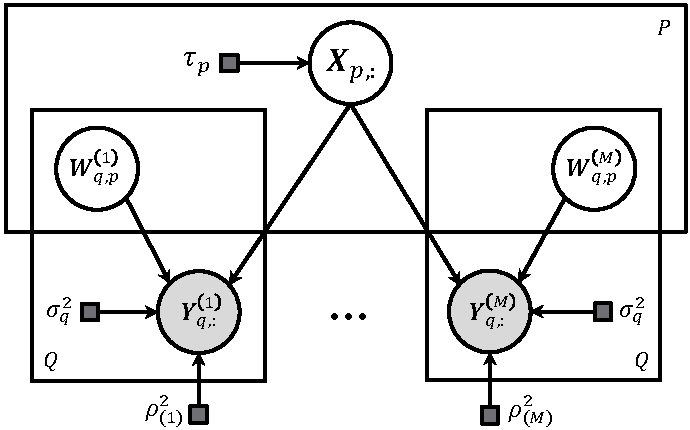
\includegraphics[width=.8\linewidth]{figures/ch1/unfold_M.pdf}
        \caption{\footnotesize Graphical Model for S-GPFA.} \label{fig:model}
    \end{minipage}
    \begin{minipage}[c]{.5\textwidth}
        \savebox\strutbox{$\vphantom{\dfrac11}$}
        \begin{align*}
            & \X_{p, :} \sim \mathcal{GP}\left(0, \kappa_p(.,.) \right) \\
            & \w{m}_{q,p} \sim \mathcal{N}(0, 1) \\
            & \Y{m}_{:, t} | \X_{:, t}, \w{m} \sim \mathcal{N} \left( \w{m} \X_{:, t}, \spcov{m} \right) \\
            & \kappa_p(t_1, t_2) = \exp \left( -\frac{(t_1 - t_2)^2}{2\tau_p^2} \right)
        \end{align*}
  \end{minipage}
    \vspace{-1em}
\end{figure}

\sloppy To find the model parameters, we employ gradient ascent (using ADAM optimizer \cite{adam} and TensorFlow Probability) to maximize the joint probability distribution of observations and latent variables, conditioned on model parameters. The collective set of model parameters and latent variables to be inferred is denoted by $\params=\Bigl\{ \X, \{\w{m}, \sv{m}\}_{m=1}^M, \{\rv{q}\}_{q=1}^Q, \{\tau_p\}_{p=1}^P \Bigr\}$. The resulting maximum a posteriori (MAP) estimate of model parameters is the minimizer of the objective function in (\ref{eq:nll}):

\begin{align} \label{eq:nll}
    % \hat\params = & \underset{\params}{\operatorname{argmin}} \nonumber \\
    & \sum_{m=1}^{M} \sum_{q=1}^{Q} \left[ \frac{T}{2} \log(2\pi\sv{m}\rv{q}) + \frac{\norm{ \Y{m}_{q,:} - \w{m}_{q,:} \X }^2}{2\sv{m}\rv{q}} \right]   \\
    + & \frac{\lambda}{2} \sum_{p=1}^{P} \left[\log\det(2\pi \K_{p}) + \X_{p,:} \K_{p}^{-1} \X_{p,:}^T \right]
    % \nonumber \\
    + \sum_{m=1}^{M} \frac{1}{2} \norm{\w{m}}_F^2 
     \nonumber
\end{align}

where $\norm{\cdot}_F$ denotes the Frobenius norm. For now, let us set $\lambda=1$ to achieve the standard MAP solution -- we will explain the motivation behind including such constant in the objective function later in this section. The first summation term in (\ref{eq:nll}) is the reconstruction loss promoting data fit. We refer to the second summation term as the smoothness loss, where $\log\det(\K_p)$ constitutes a model complexity penalty (in terms of smoothness) and $\X_{p,:} \K_{p}^{-1} \X_{p,:}^T$ promotes smooth latent trajectories governed by $\tau_p$. Finally, the last term is a weight decay loss for subjects' factor loadings. While the reconstruction loss favors complex models to fit the observed data, smoothness and loadings weight decay losses act as regularizers to promote smooth and less flexible models, respectively.

Increasingly, fMRI studies include sample sizes of hundreds of participants ($M$) with thousands of voxels recorded ($Q$). An examination of the objective function in (\ref{eq:nll}) reveals that the objective is extensively dominated by the reconstruction loss, since the total number of observed time series, $Q M$, is often orders of magnitudes larger than the latent space dimensionality $P$. In such a case, the solution of (\ref{eq:nll}) cannot afford to model the temporal smoothness properties of the data, and consequently, attempts to fit the observed data with a possibly complex model. To resolve this issue, we amplify the smoothness loss in (\ref{eq:nll}) by hyperparameter $\lambda \propto \m\q/\p$ to balance the weight of the smoothness loss against the reconstruction loss. Note that from a probabilistic perspective, such regularization can be interpreted as weighted likelihood \cite{weightedlikelihood}. Although, as with any hyperparameter, standard methods like cross validation can be employed to tune $\lambda$, we use the fixed value of $0.1 \times \m\q/\p$ for all experiments conducted in the present paper. 

\sloppy Adding a new subject $\m+1$ to a previously trained model is done through finding the maximizer of $\text{P}(\Y{\m+1}, \w{\m+1} | \X, \sv{\m+1},  \{\rv{q}\}_{q=1}^Q)$ with respect to $\w{\m+1}$ and $\sv{\m+1}$. Note that the shared latent trajectories, existing subject's topographies, and region/subject noise factors will remain unchanged.
In addition, using previously learned topographies, shared timescales, and noise factors, one can map new observations from the existing subjects in the training cohort into the shared space. This can be done by maximizing 
$\text{P}(\{\y_{\text{new}}^{(m)}\}_{m}, \X_{\text{new}} | \{\w{m}, \sv{m}\}_{m}, \{\rv{q}\}_{q=1}^Q, \{\tau_p\}_{p=1}^P)$
with respect to $\X_{\text{new}}$, where $\y_{\text{new}}$ denotes new observations from the subjects in the training cohort and $\X_{\text{new}}$ shows the associated shared latent trajectories. 


\section{Results}
\label{sec:experiments}

We present two sets of experiments to demonstrate the utility of S-GPFA. First, using the Raider datasets \cite{ha}, we perform the time segment matching experiment to measures generalization of learned temporal dynamics and topographies to unseen subjects and observations. In the second experiment, we apply our model to another multi-subject dataset (SPINS \cite{spins}), allowing us to evaluate and interpret topographies and group-specific temporal dynamics. 
% Further details of both datasets has been published by original study authors \cite{ha, spins}.
% Taken together, our experiments show the proposed model can achieve equal performance in terms of aggregating subjects' observations, by employing temporal information already available in data, without the need for imposing unrealistic modeling assumptions. 

\subsection{Time Segment Matching}
A time segment matching experiment, as first introduced by \cite{ha}, can evaluate how shared dynamics found by S-GPFA generalizes to new subjects and unseen data. We follow the modified version of the experiment presented in \cite{srm}, where the task is to locate an unseen segment of a test subject's response in time. We partition the fMRI dataset in time into two equal-size parts and leave one subject out to use the remaining subjects as training participants. We shall note the four resulting parts as \ytrain{1}, \ytest{1}, \ytrain{2}, and \ytest{2}.

As shown on the top diagram in Figure \ref{fig:tsm}, the first half of the data is used to learn subject-specific topographies. First, an S-GPFA model is fit to the first half of training subjects' data \ytrain{1}, to learn shared latent trajectories \xtrain{1} and subject-specific topographies \wtrain. Next, using the learned shared trajectories \xtrain{1} and the first half of test subject's data \ytest{1}, topographies for the held-out subjects \wtest is calculated, as discussed in section \ref{subsec:model}. The second half of data is used for measuring time segment matching accuracy. More specifically, given the second half of training subjects' data, \ytrain{2}, we wish to locate an unknown segment from the held-out subject's data \yseg in time. By only using the raw observations as a baseline, one can first find the average response of training subjects, then report the time where \yseg and the average response are maximally correlated. Moreover, using learned subject topographies, we can transform \ytrain{2} and \yseg into the shared space using \wtrain and \wtest as discussed in section \ref{subsec:model}, to find \xtrain{2} and \xseg. Using a similar correlation classifier, we can locate the test segment in the point where \xtrain{2} and \xseg are maximally correlated. Figure \ref{fig:tsm} compares the time segment matching accuracy for different query segment lengths. S-GPFA demonstrates similar performance as SRM in terms of time segment matching accuracy. This posits that shared temporal dynamics (timescales) found in training subjects can be generalized to new subjects with unseen observations. 

\begin{figure}[tb!]
    \centering
    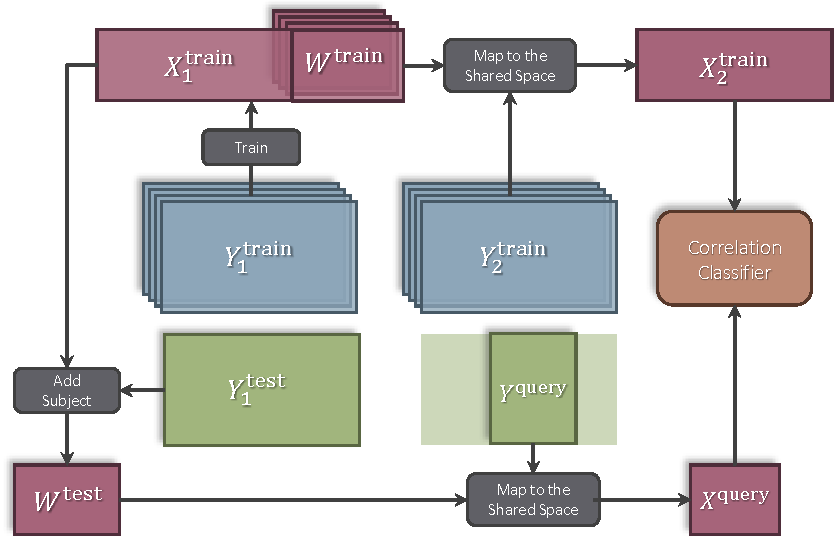
\includegraphics[width=.5\linewidth]{figures/ch1/tsm_blockdiagram.pdf}
    \vspace{1em}
    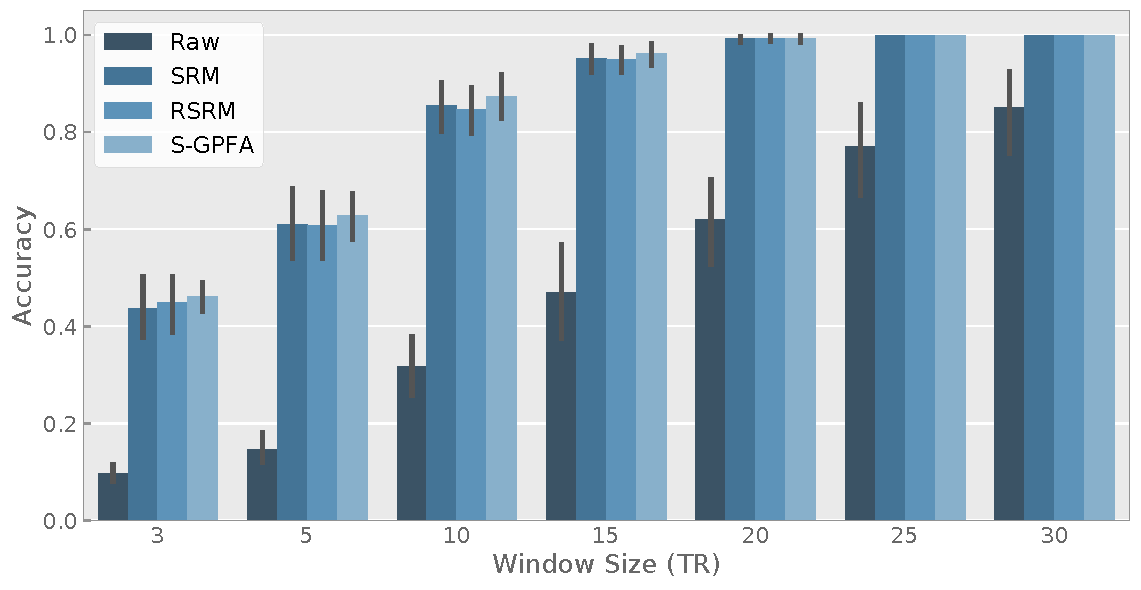
\includegraphics[width=.6\linewidth]{figures/ch1/tsm_raider_p10_sm200_2.pdf}
    \caption{Time Segment Matching Experiment. Top: schematic procedure of the experiment. Bottom: Time segment matching accuracy for Raider dataset (10 subjects, first 400 TRs). We used $P= 10$ for SRM, RSRM, and S-GPFA. Error bars show $\pm$ standard deviations.}
    \label{fig:tsm}
\end{figure}

\subsection{Application: SPINS Dataset}

\begin{figure*}[!t]
    \centering
    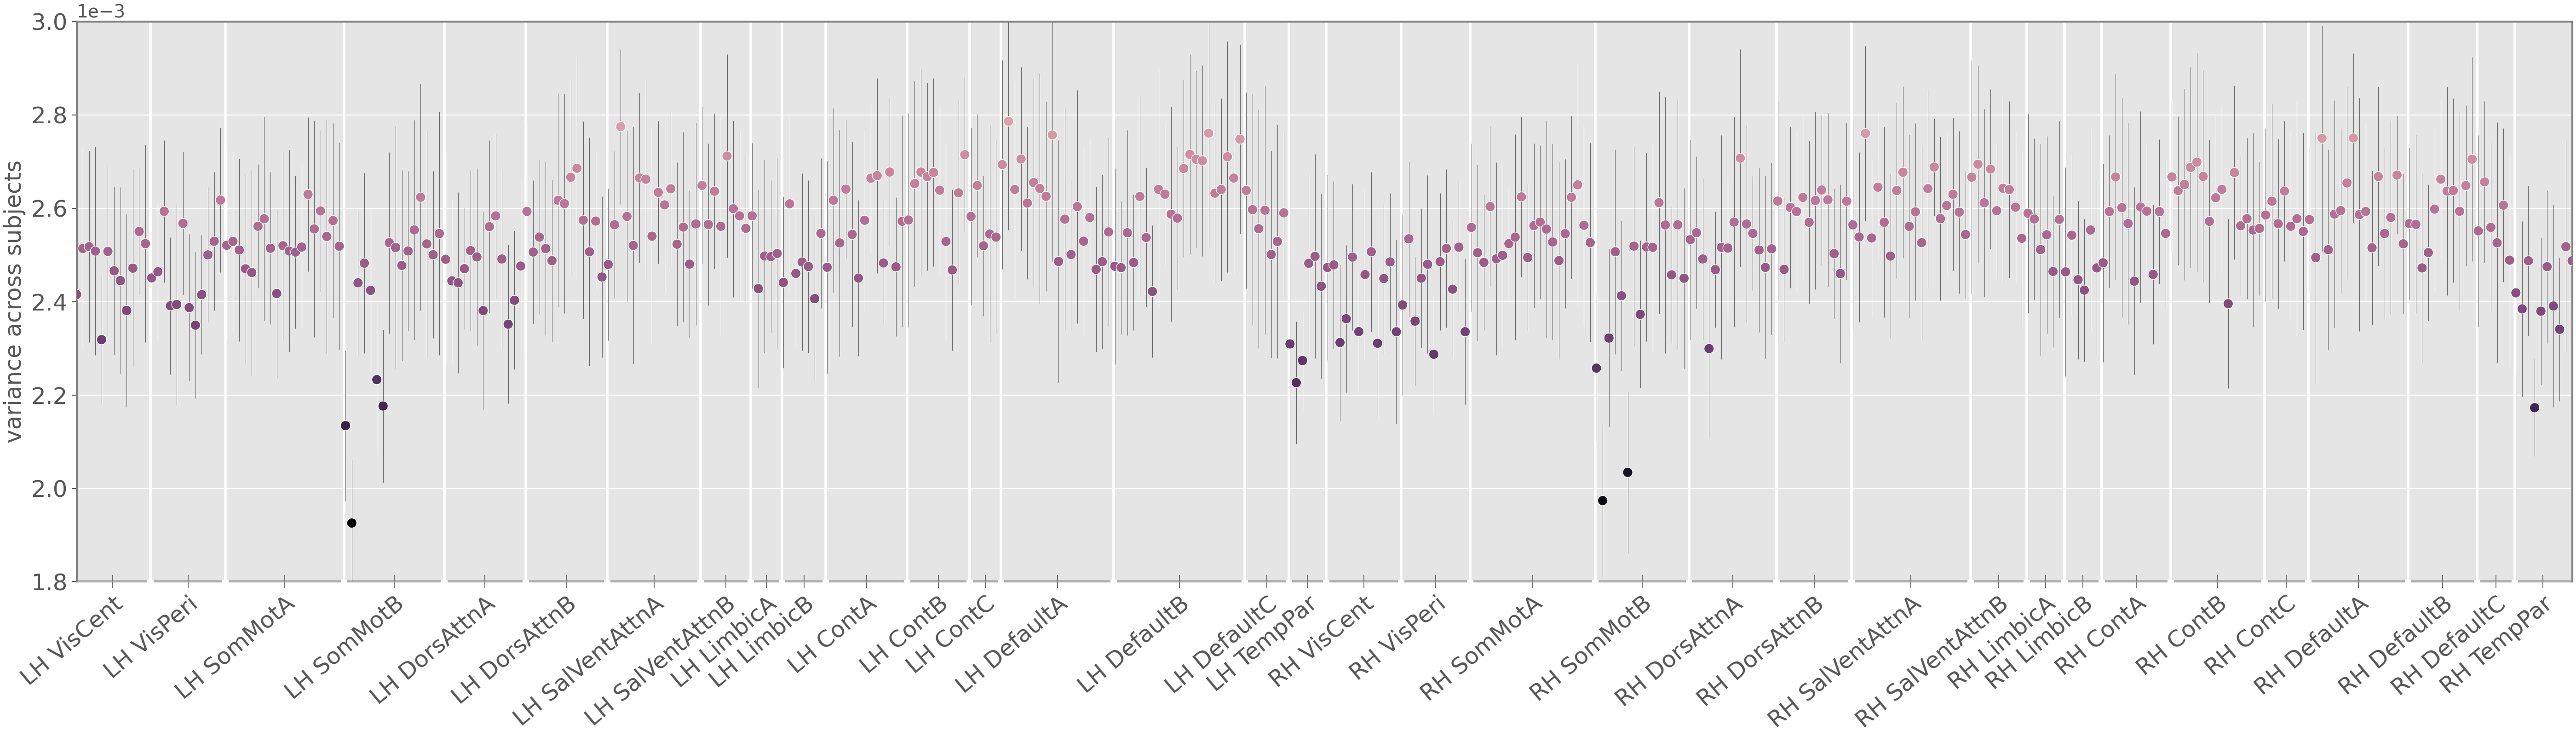
\includegraphics[width=1\linewidth]{figures/ch1/topo_cons_scatter.png}
    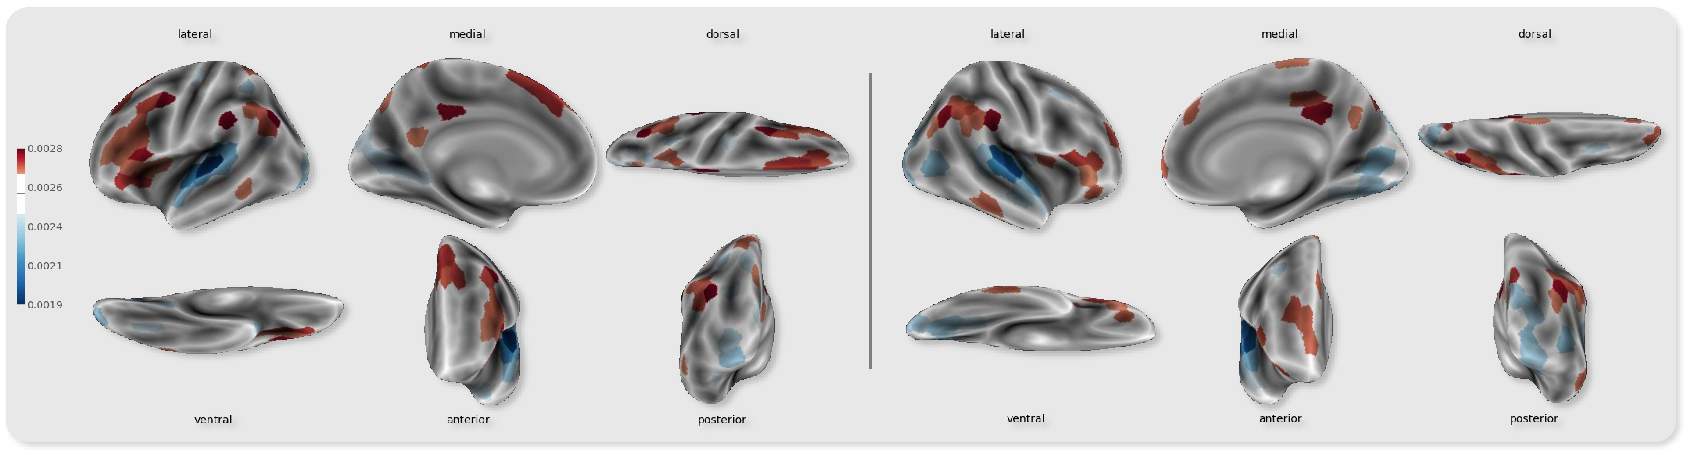
\includegraphics[width=1\linewidth]{figures/ch1/topo1_brain.pdf}
    \caption{Top: Variance of normalized $\p=20$ topographies across subjects (Y axis) for different regions (X axis). Regions are divided into 17 Yeo sub-networks \cite{yeo}. Colored dots indicate the mean (across different topographies) of variances for each region, and error bars shows $\pm$ standard deviation. Bottom: Brain surface plots of average variance of normalized topographies, for left and right hemispheres. Blue (red) indicates higher (lower) consistency across subjects. 
    % In both panels, the second of nine EA videos is shown: all videos showed comparable patterns.
    % See Supplementary Materials (section \ref{sec_suppmat:topo_consistency}) for other EA videos.
    }
    \label{fig:topo}
\end{figure*}

For our final set of experiments, we applied S-GPFA to a subset (332 subjects) from the NIMH Data Archive study “Social Processes Initiative in the Neurobiology of the Schizophrenia(s)” (SPINS) who completed the Emotional Accuracy (EA) task. The EA task collects fMRI as participants watch videos of an actor (‘target’) recounting autobiographical events. In total, 9 videos were shown, lasting for between 2-2.5 minutes. Participants provide ratings of the target’s valence on a 9-point scale (1=extremely negative, 9=extremely positive) in real time via button press. The tasks' primary dependent measure, the EA score, is the correlation between the participant’s ratings of the targets’ emotions, and the “gold standard” rating of the targets’ ratings of their own emotions, calculated in 2 second time epochs. We selected SPINS as an experimental dataset because it includes participants with and without schizophrenia, and we held that the anticipated variability in brain structure, function, and cognitive performance would provide an interesting test of S-GPFA.

\textbf{Consistency of Functional Topographies - }
In our first analysis, we examined whole-brain variation in activation during the EA task, across all subjects. Learned factor loading matrices $\W$ in S-GPFA are, by model definition, subject-specific basis vectors that generate each subject's observation from a shared set of latent trajectories: $\w{m}\X \simeq \Y{m}$. Therefore, columns of factor loadings $\{\W_{:,p} \in \reals^\q\}_{p=1}^{\p}$, for different subjects, are perturbed versions of an activation template. This allows the model to capture functional variability across subjects. Hence, we can examine the amount of subject variability in each individual brain region of interest (ROI) for a given task, by looking at the variance of learned topographies over participants. To this end, for every topography $p$ of subject $m$, we first normalize $\w{m}_{:,p}$, then we find the variance of these normalized topographies over subjects. This will result in $\p$ variance values for each of $\q$ regions indicating a measure of subject variability, as shown in Figure  \ref{fig:topo}. Note that, for the present analysis, we used cortical parcellations from the Schaefer atlas (400 ROIs) \cite{schaefer2018local} grouped in accordance with the Yeo17 parcellation \cite{yeo}. 

Examination of subject variance in functional topography itself shows variability across ROIs. Perhaps unsurprisingly, the lowest variance (blue) is evident in the motor network, engaged similarly by the task’s continuous button-press demands, and in temporal lobe areas related to audition, engaged by the audio aspect of the task. Excitingly, we see lower consistency (red) in the distributed frontal-parietal (‘Control A’) network, which contains the inferior frontal gyrus (IFG) and inferior parietal lobule (IPL), that together constitute the canonical human mirror neuron system \cite{iacoboni2006mirror}. That we were able to identify high variability in a network believed to subserve social cognition provides an important proof of principle that S-GPFA is able to identify meaningful variance within a heterogeneous sample. We expect that S-GPFA will enable important tests of both exploratory and hypothesis-driven examinations of functional topography in psychiatric disorders.

\begin{figure}[tb]
    \centering
    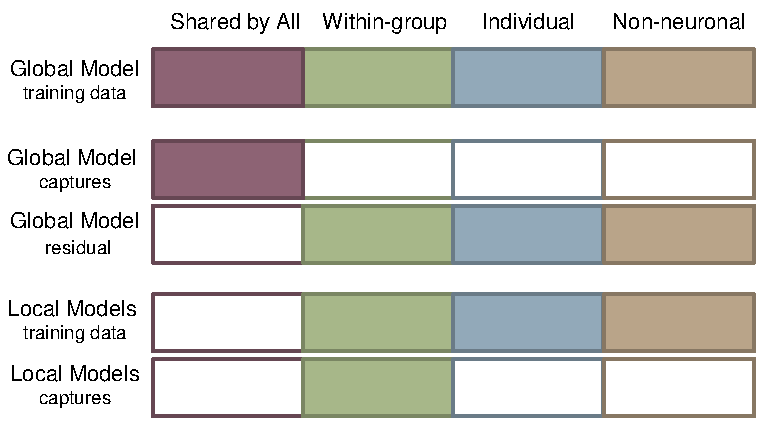
\includegraphics[width=.5\linewidth]{figures/ch1/group_tf_schematic_2.pdf}
    \vspace{0.4em}
    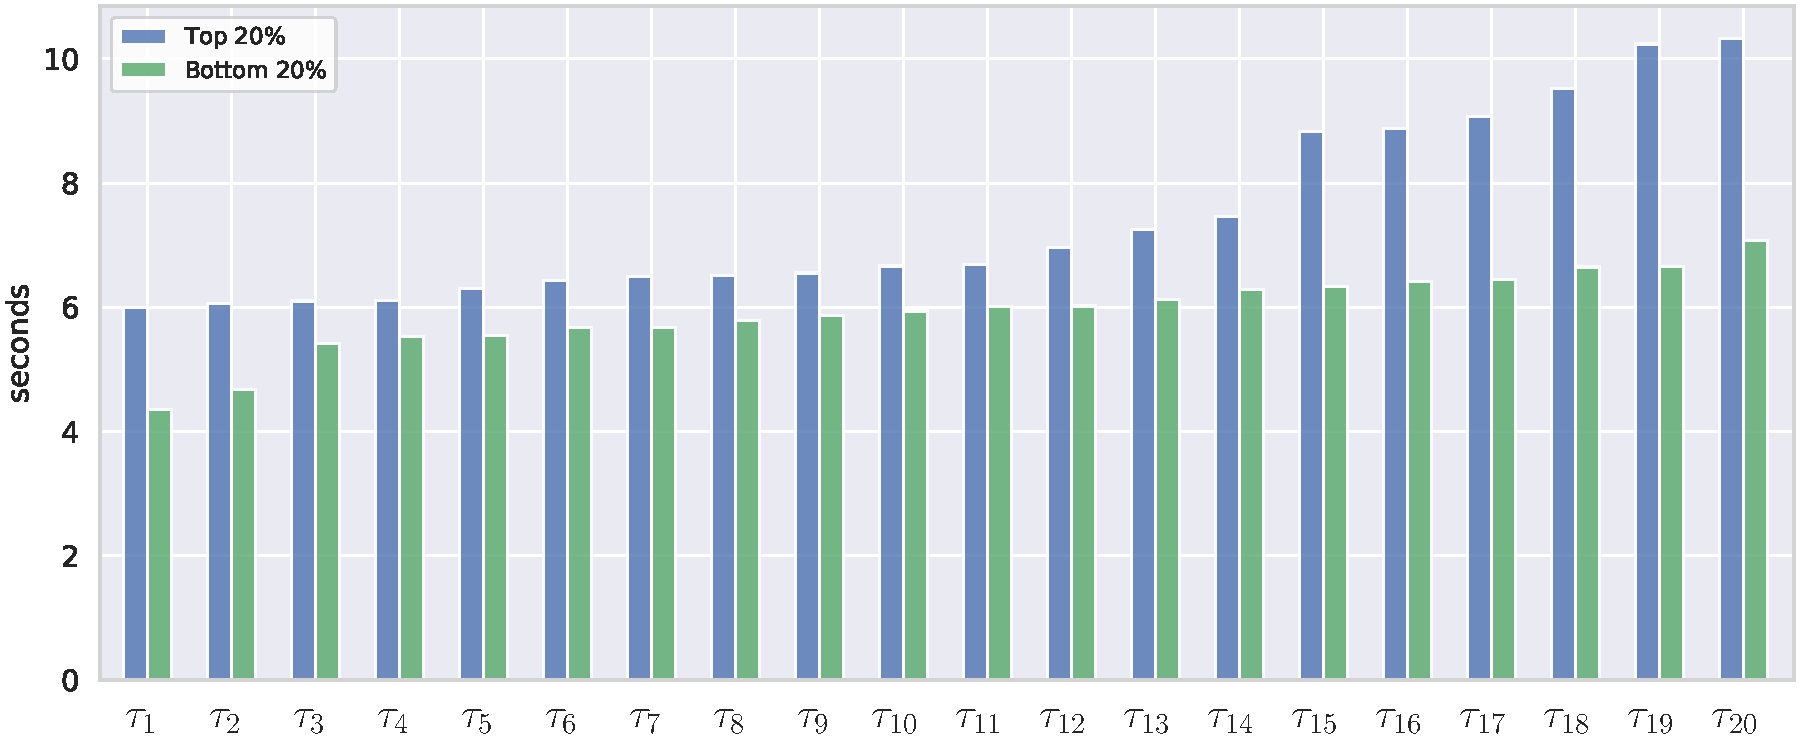
\includegraphics[width=0.9\linewidth]{figures/ch1/group_td.pdf}
    \caption{Top: Different data components captured using the global and local models. Bottom: Group-specific timescales (sorted by magnitude) discovered using local models, after removing temporal patterns shared across all subjects.}\label{fig:gtd}
\end{figure}

\textbf{Group-specific Temporal Dynamics - }
Next, we employed S-GPFA to examine group-specific temporal dynamics. Our method is illustrated in Figure \ref{fig:gtd} (top). First, a \textit{global} model is trained using subjects from all groups. Residuals of the global model, as defined by $\Y{m} - \w{m} \X$, for $m \in \{1, \ldots, \m \}$, allow us to remove components of the observations that are shared among all groups \cite{srm}. Next, separately on each group, two models are trained over the residuals of the global model. These \textit{local} models capture group-specific dynamical components in observations after the globally shared components of the data are removed. 

We applied this approach to the SPINS dataset, opting to split the sample into two smaller groups comprised of individuals demonstrating EA scores within the top and bottom 20th percentiles, respectively. This bifurcation allowed us to isolate subjects with distinctly strong and poor socioemotional cognition, irrespective of schizophrenia diagnosis \cite{insel2014nimh}. Figure \ref{fig:gtd} (bottom) shows group-specific timescales discovered via the local models, after extraction of the residuals from the global model, i.e., after all signals with a global structure have been removed. In the local models, we observe that the group with the strongest EA performance shows less temporal variability, i.e., the dynamical patterns in those individuals with the greatest socioemotional cognitive capacity unfolded over slower timescales, in contrast to those participants with comparatively impoverished capacity. This observation is consistent with broad evidence of a relationship between domain-specific task performance, and observed modularity versus flexibility of task-relevant brain networks, e.g.\cite{olsen2013functional}, and the recent dissociation that strong performance on tasks involving little executive function or cognitive control (consistent with EA task demands) may be subserved by modular network activation \cite{ramos2017static}. Importantly, the isolation of low-dimensional group-specific timescales allows for the identification of differences of small effect, which may be statistically occluded in global models. 




\section{Future Plans} % Import your chapters here
% \chapter{Distributed Coded Training on the Cloud} \label{ch-2}



\section{Experimental results}
\label{sec:experiments}

In this section, we evaluate the performance of proposed schemes by training multiple neural network models concurrently. We use the AWS Lambda,
% \footnote{https://aws.amazon.com/lambda/}
a fully-managed and cost-efficient serverless cloud computing service. Workers are invoked from the master node using HTTP requests, and task results are received in the HTTP response payload. Appendix~\ref{sec:lambda} provides a detailed discussion of our network setup and cloud resources.

\subsection{Analysis of response time}
\label{subsec:response-time}

Our experiment setup consists of a master node and $n=256$ workers. In Fig.~\ref{fig:4-1}, we demonstrate statistics of response time across $100$ rounds, where each worker calculates gradients for a batch of $16$ MNIST images on a CNN involving three convolutional layers, followed by two fully connected layers.  Fig.~\ref{fig:4-1}(a) shows the response time of each worker at every round. White cells represent stragglers. As discussed in Sec.~\ref{sec:setting}, a worker is deemed straggler when its response time exceeds $(1+\mu)$ times the response time of the fastest worker in the round. For the sake of consistency, we choose $\mu=1$ for all experiments. Nonetheless, such a choice of $\mu$ is by no means critical to observe stragglers. This can be seen in Fig.~\ref{fig:4-1}(c), where the empirical CDF of workers' completion time exhibits a relatively long tail. Fig.~\ref{fig:4-1}(b) plots the number of straggler bursts of different length over this response profile. It can be observed that our response profile does not include nodes that continue to remain stragglers for long duration. This motivates the use of coding across the temporal dimension as proposed in the present work.


\begin{figure}[h]
    \centering
    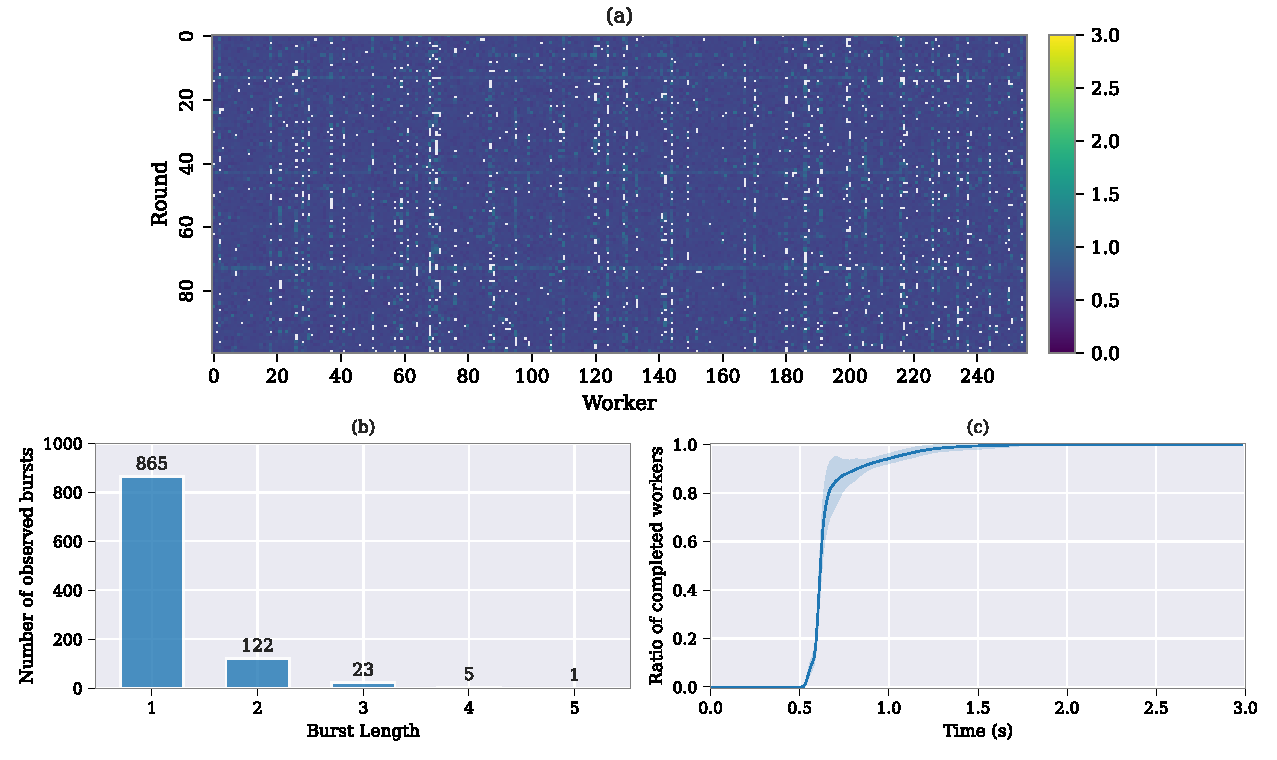
\includegraphics[width=\textwidth]{figures/ch2/fig1.pdf}
    \caption{Statistics of response time for 256 workers across 100 rounds. Each worker calculates gradients of the loss for a batch of 16 MNIST images on a convolutional neural network. (a) Each white cell represents a worker (x-axis) who is a straggler at the corresponding round (y-axis). (b) Histogram of stragglers' burst lengths. (c) Empirical CDF of workers' completion time, averaged over 100 rounds (shades represent standard deviation).}
    \label{fig:4-1}
\end{figure}

\subsection{Comparison of coding schemes}

Using the setup described in Sec.~\ref{subsec:response-time}, we train $M=4$ CNN classifiers for MNIST concurrently following the approach stated in Remark \ref{rem:job_dependency}. In every round, master samples a batch of $4096$ data points and distributes them among the workers. Non-straggling workers compute partial gradients and return task results to the master at the end of each round. After completion of one update, master uploads the updated model parameters to a shared network file system, accessible to the workers.  We use cross entropy as the loss function and ADAM as the optimizer. Moreover, the same dataset and architecture are used for all the models.

In each experiment, we run a total of $J=480$ jobs (120 jobs per classifier) using the three schemes, namely GC, SR-SGC and M-SGC. As a baseline, we also train the classifiers without any coding wherein the master node should wait for all the workers to return their task results. Finally, each experiment is repeated 10 times to report the first and second-order statistics of total run times. Before training the models, we perform some shorter experiments to choose the best-performing parameters for each of the three coding schemes. Specifically, for GC, we perform a grid search over $s$ and select the value corresponding to the shortest run time. We refer readers to Appendix~\ref{sec:param_selection} for the exact procedure of selecting the parameters for SR-SGC and M-SGC schemes.
% \textcolor{blue}{We should at least explain here why $s=15$ for GC was chosen} 

Table \ref{table:4-1} presents the total run time achieved by each coding scheme, along with the selected parameters and resulting normalized loads.
Selection of small values for parameters $B$ and $W$ in our sequential coding schemes matches the empirical evidence in Fig.~\ref{fig:4-1}(b) that isolated short-length-bursts are prevalent. It is interesting to note that the effective value of parameter $s$ in SR-SGC ($s=12$) turns out to be close to that of GC ($s=15$).  Fig.~\ref{fig:4-2}(a) plots total number of completed jobs (for all $M=4$ models) across time, and Fig.~\ref{fig:4-2}(b) shows the course of training loss (of the first model out of the $4$ models) as a function of  time, for all coding schemes. 

\vspace{-0.5em}
\begin{table}[h]
\caption{Total run time achieved by different coding schemes} \label{table:4-1}
\vspace{-1em}
\begin{center}
\begin{tabular}{lccl}
\multicolumn{1}{c}{\bf Scheme}  &\multicolumn{1}{c}{\bf Parameters} &\multicolumn{1}{c}{\bf Normalized Load} &\multicolumn{1}{c}{\bf Run Time (s)} 
\\ \hline \\
M-SGC	   	&$B=1, W=2, \lambda=27$	&$0.008$    &$891.37 \pm 43.10 $\\
SR-SGC	   	&$B=2, W=3, \lambda=23 \; \ (s=12)$	&$0.051$    &$994.22 \pm 43.66 $\\
GC	       	&$s=15$	                &$0.062$    &$1064.96 \pm 46.72$ \\
No Coding	&$-$	                &$0.004$    &$1307.79 \pm 61.88$ 
\end{tabular}
\end{center}
\end{table}
\vspace{-1.5em}

\begin{figure}[h]
    \centering
    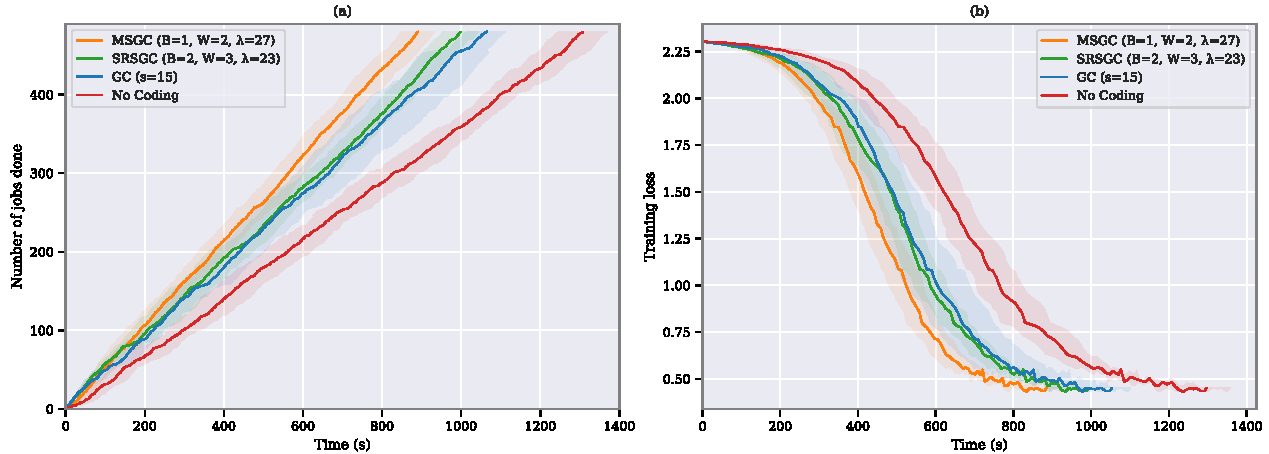
\includegraphics[width=\textwidth]{figures/ch2/fig2.pdf}
    \caption{(a) Number of completed rounds vs. clock time, averaged over 10 independent experiments. (b) Training loss vs. clock time for the first model (out of four concurrently trained models), averaged over 10 independent runs. Shades here represent standard deviation.}
    \label{fig:4-2}
\end{figure}

The first clear observation from Table \ref{table:4-1} is that our proposed M-SGC achieves 16\% lower run time while maintaining smaller normalized load compared to the classical GC scheme. Furthermore, compared to GC, SR-SGC shows slight improvements in total runtime and normalized load simultaneously, demonstrating the potential of incorporating selective repetition into GC. Next, as shown in Fig.~\ref{fig:4-2} and Table \ref{table:4-1}, the existence of stragglers is validated by the fact that any of the coding schemes significantly outperforms the case of not using any coding. This is indeed in line with the empirical observation of Figure \ref{fig:4-1}(c), where the tail of the cumulative distribution of workers' completion time signals the existence of stragglers.





\section{AWS Lambda architecture}\label{sec:lambda}

This section discusses the overall architecture, limitations, and additional details about the setup and usage of the AWS cloud resources used in our experiments (Sec.~\ref{sec:experiments}). 

We use AWS Lambda functions as workers in our distributed training experiments. Each Lambda instance has $2500$ MB of RAM, $1$ vCPU, and supports Python 3.8 runtime environment. A Lambda layer is used to inject external dependencies into the runtime environment (e.g. PyTorch, TorchVision, NumPy etc). Since the size of required external libraries exceeds the 200MB limit of Lambda layers, we zip some libraries in the layer package and unzip them at the time of Lambda instance creation. Note that this will not affect workers' run times as we perform a \textit{warm-up} round before each experiment to ensure that our Lambda instances are initialized and functional. 

Another limitation concerning the use of Lambda functions for training ML models is the total payload size quota of $6$ MB. i.e., the total sum of payload sizes in the HTTP request and response cannot exceed $6$ MB. Note that ideally the master includes current model weights in the HTTP request payload, and receives the task results via the HTTP response payload. This incurs a serious limitation on any reasonably-sized neural network. To overcome this, we need to use a proxy storage service to communicate model weights and task results.

Fortunately, we have two storage options; Amazon S3 (Simple Storage Service) and AWS EFS (Elastic File System). We use the latter, as it will provide higher throughput. EFS is a shared network file system that will be mounted on all Lambda instances at their time of creation. This way, it can be used as a means for communication between the master and workers. In our experiments, we reserve the payload limit for the task result communication, and use EFS to communicate updated model weights to workers, as depicted in Figure \ref{fig:aws} (a). The overall architecture of our cloud resources is shown in Figure \ref{fig:aws} (b). We use AWS Serverless Application Model (SAM) tool to define, manage, and deploy the cloud resources (included in the code submitted as supplementary material).  

\begin{figure}[h]
	\centering
	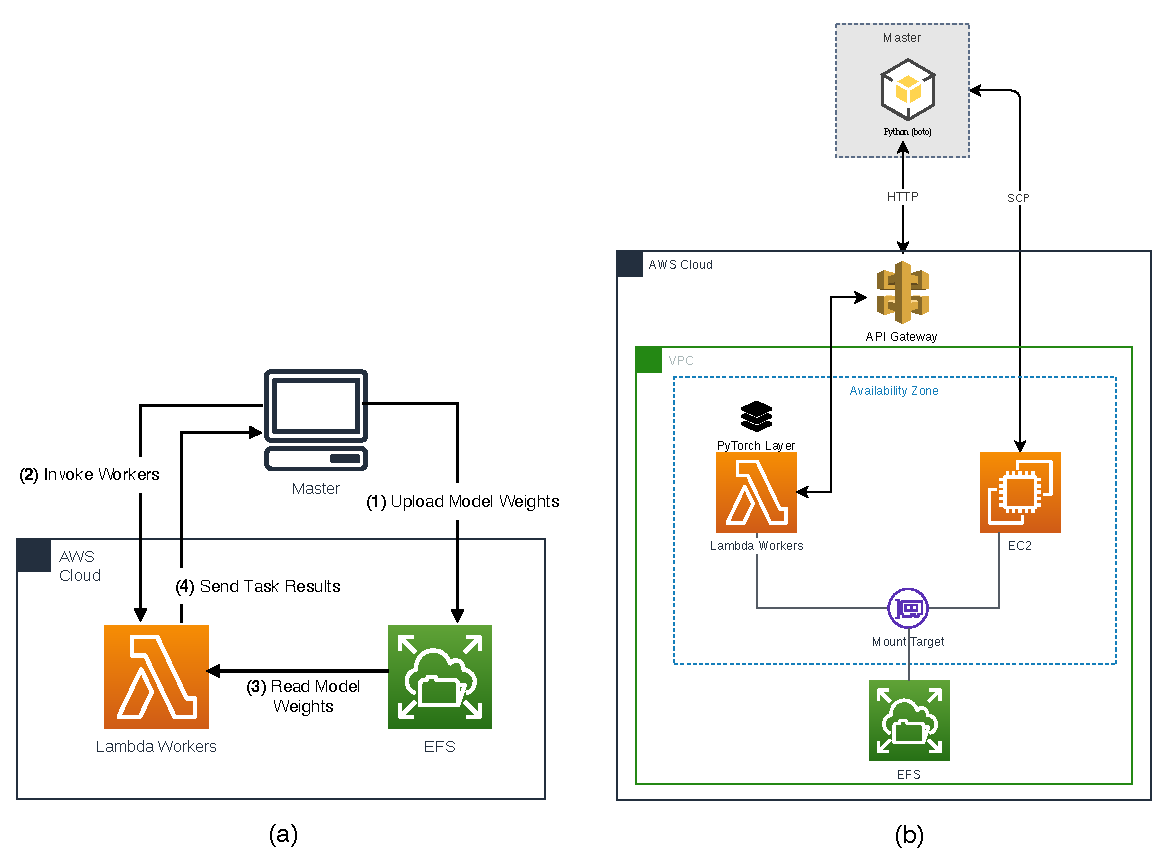
\includegraphics[width=\textwidth]{figures/ch2/aws.pdf}
	\caption{(a) Communication between master and Lambda workers for each round. (b) The overall architecture of AWS cloud resources used.}
	\label{fig:aws}
\end{figure}

\section{Selecting coding scheme parameters}\label{sec:param_selection}

This section discusses the parameter selection method used for our proposed sequential gradient coding schemes, SR-SGC and M-SGC. We begin by noting that the total number of valid parameter combinations for each of these schemes are too large for a grid search to be feasible, as evaluation of each parameter combination requires training models for multiple rounds. Instead, we utilize the observation that increasing the normalized load will linearly increase the average runtime of the workers. Fig.~\ref{fig:base_comp} shows the average runtime of 256 workers across 100 rounds for some values of load $\in [0, 1]$. 

\begin{figure}[h]
	\centering
	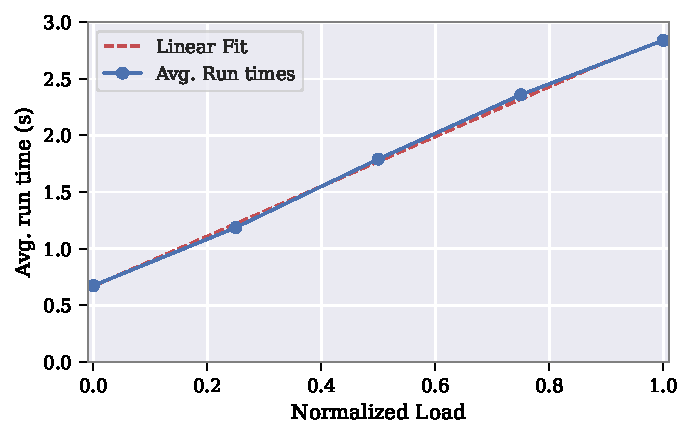
\includegraphics[width=0.45\textwidth]{figures/ch2/5.pdf}
	\caption{Average run time scales linearly with increase in workers' computational load.}
	\label{fig:base_comp}
\end{figure}

We can exploit the observation above to estimate the delay profile corresponding to various coding schemes with variable normalized loads. After estimating the slope of linear fit in Fig.~\ref{fig:base_comp} (let this be $\alpha$), we run our distributed training experiment for $80$ jobs with no coding, and store the observed runtime of workers across rounds (we call this the \textit{reference delay profile}). The normalized worker load in case of no coding will be $1/n$. 
Next, considering a coding scheme with fixed parameters (and therefore a fixed load $l$), we opt to feed this profile to the master node to simulate the run time of workers. However, note that we have to take into account the increase in the workers' run time due to the increase of the load from $1/n$ to $l$. Based on our previous discussion, we can compensate for this increase by adding $(l - 1/n) \alpha$ seconds to our reference delay profile. Using this \textit{translated} delay profile, and based on the assumed coding scheme, the master node will try to resolve stragglers at each round, and if not, it will wait out all the workers, resulting in a simulated total run time for the coding scheme. Fig.~\ref{fig:allparams} shows the result of the above procedure for all valid parameter combinations of SR-SGC and M-SGC. 

\begin{figure}[h]
	\centering
	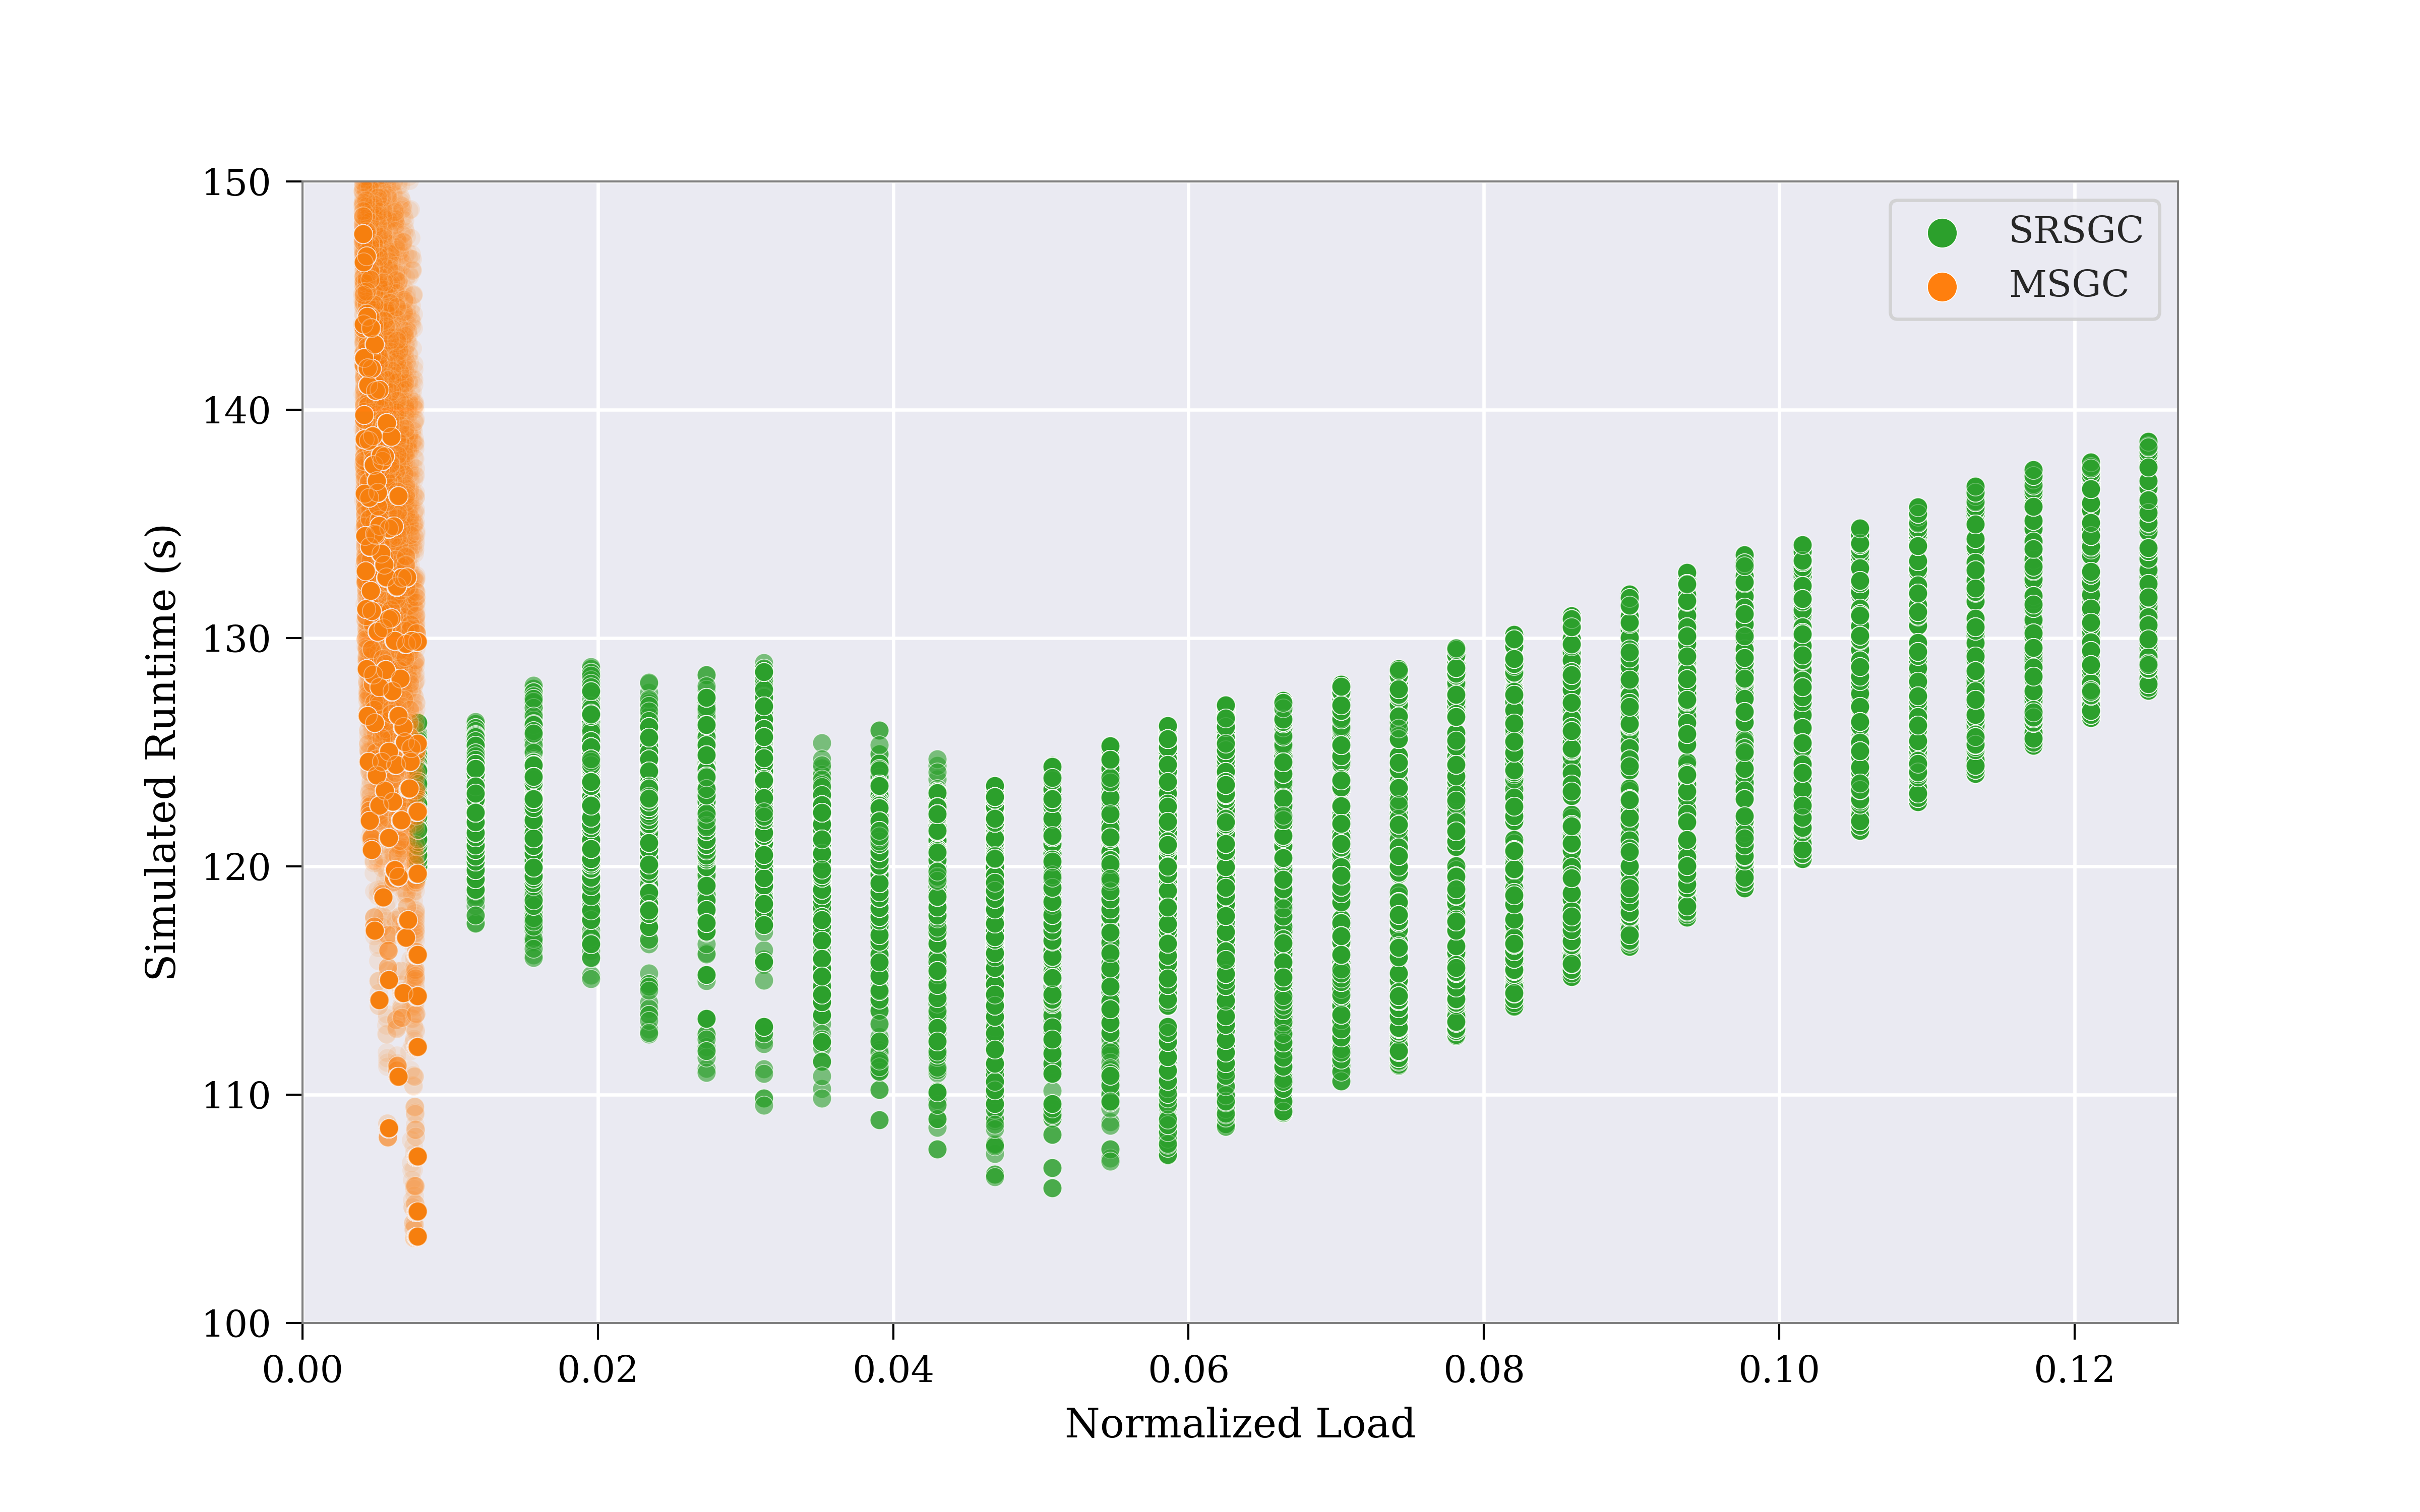
\includegraphics[width=0.65\textwidth]{figures/ch2/6.png}
	\caption{Simulated total run times of calculating 80 jobs using SR-SGC and M-SGC. Each point represents one parameter combination.}
	\label{fig:allparams}
\end{figure}

	For each of the two schemes, we select the parameters corresponding to the smallest total run time. The selected parameters are stated in Table \ref{table:4-1}. Note that as per Remark \ref{rem:comp_load_comparison}, normalized load of M-SGC is upper-bounded by $2/n$, which can also be observed in Fig.~\ref{fig:allparams}.




\section{Problem Definition}

\section{Outcomes}

\section{Future Plans}

\chapter{Entropy-based Lossy Compression} \label{chap-3}

\section{Problem Definition}

Let us consider the following general lossy compression setup:

\begin{equation}
    X \xrightarrow{\enc(T|X)} T \xrightarrow{\dec(Y|T)} Y
\end{equation}

where input $X$ with marginal distribution $P_X$ is encoded using the probabilistic encoder $\enc$ to generate code $T$. In turn, the probabilistic decoder $\dec$ reconstructs $Y$ from the code $T$. The goal is to find the encoder and decoder that minimize the expected code length $H(T)$, given a distortion constraint on $Y$. It is common to measure the sample-wise distortion via direct comparison of $(x, y)$ pairs through a distortion function $d(\cdot, \cdot)$, and consider the expectation as a notion of overall distortion, $\ex \left[ d(X,Y)  \right]$. Instead, we will consider log-loss $H(X|Y)$ as an alternative to enforce distortion constraint. Therefore, the optimization problem can be stated as follows:

\begin{equation}
\begin{aligned} \label{eq:no_const}
    \min_{\enc, \dec} \ &H(T)\\
    \textrm{s.t.} \ &H(X|Y) \leq \theta
\end{aligned}
\end{equation}

It is easy to see the optimal solution of (\ref{eq:no_const}) happens when $T=Y$, i.e. the identity decoder. To overcome this we constrain the output marginal distribution:

\begin{equation}
\begin{aligned} \label{eq:no_const}
    \min_{\enc, \dec} \ &H(T) \\
    \textrm{s.t.} \ &H(X|Y) \leq \theta \\
    &P(Y) = P_Y
\end{aligned}
\end{equation}

or equivalently:

\begin{equation} 
\begin{aligned} \label{eq:general}
    \min_{\enc, \dec} \ &H(T) - \beta I(X;Y) \\
    \textrm{s.t.} \ &P(Y) = P_Y
\end{aligned}
\end{equation}

A special case of (\ref{eq:general}) is when the code bottleneck is removed, i.e. $\beta \to \infty$. In this case, $X=T$ and the optimization becomes:

\begin{equation} 
\begin{aligned} \label{eq:maxmutual}
    \max_{\enc} \ &I(X;Y) \\
    \textrm{s.t.} \ &P(Y) = P_Y \\
\end{aligned}
\end{equation}

That is, finding the probabilistic pairing between the marginals $P_X$ and $P_Y$ in order to maximize the mutual information. We refer to (\ref{eq:maxmutual}) as the \textit{Maximum Information Matching} problem.


\section{Maximum Information Matching}

Consider two random variables $X$ and $Y$, over alphabets $\mathcal{X}$ and $\mathcal{Y}$ with probability mass functions $P_X$ and $P_Y$, respectively. The goal of Maximum Information Matching is to find the joint probability mass function $P_{XY}$ that maximizes the mutual information $I(X;Y)$, or equivalently minimizes the joint entropy $H(X;Y)$:

\begin{equation} 
\begin{aligned} \label{eq:minent}
    \min_{P_{XY}} \ &H(X;Y) \\
    \textrm{s.t.} \
        &\sum_{y\in\mathcal{Y}} P_{XY}(x, y) = P_X(x) \quad \forall x\in{\mathcal{X}},  \\
        &\sum_{x\in\mathcal{X}} P_{XY}(x, y) = P_Y(y) \quad \forall y\in{\mathcal{Y}}
\end{aligned}
\end{equation}

This is a concave minimization problem over a standard polyhedron. Therefore, every vertex of the polyhedron is a local minimum and the global minimum happens at a subset of the vertices.

Note that an standard polyhedron is defined as $\mathcal{P}=\{\bm{x} \in \reals^n | \ \bm{A}\bm{x} = \bm{b}, \ \bm{x} \geq \bm{0}\}$, where $\bm{A} \in \reals ^{m \times n}$ with linearly independent rows. A point $\bm{x}^* \in \mathcal{P}$ is a vertex if and only if it has $n-m$ zero elements and columns of $\bm{A}$ corresponding to other $m$ non-zero elements are linearly independent. Hence, to exhaustively iterate all the vertices:
\begin{enumerate}
    \item Choose $m$ linearly independent columns $\bm{A}_{\pi(1)}, \cdots, \bm{A}_{\pi(1)}$.
    \item Let $\bm{x}_i= 0$ for all  $i \in \pi(1),..., \pi(m)$
    \item Solve the system of $m$ equations $\bm{A}\bm{x} - \bm{b}$ for the unknowns $\bm{x}_\pi(1), \cdots, \bm{x}_\pi(m)$
\end{enumerate}

Therefore a crude upper-bound on the number of vertices would be ${n \choose m}$. This is enhanced by [] to ${n-m/2 \choose m/2}$ which is still exponential in $m$. 
Next, we will show that Maximum Information Matching problem as defined in (\ref{eq:minent}) is essentially NP-Hard. This is done by reduction from another NP-complete problem, $k$-Subset-Sum.

\begin{remark} Maximum Information Matching problem of (\ref{eq:minent}) is NP-Hard.
\end{remark}
\begin{proof}
To show an optimization problem is NP-Hard, we need to show the corresponding decision problem is NP-Hard.  Given an optimization problem, a decision version is whether or not any target value $T$ is achievable. Without the loss of generality, assume $\mathcal{X} > \mathcal{Y}$. We set $T=H(Y)$, i.e. to decide if there exists a function $f: \mathcal{X}\to\mathcal{Y}$ such that $Y=f(X)$. Let's call this problem \textit{Deterministic Matching}.

Next, we show any instance of the $k$-Subset-Sum problem can be reduced to an instance of Deterministic Matching, by a polynomial-time procedure. Consider a general instance of the $k$-Subset-Sum problem: Given set $\mathcal{S}$ of integers and target values $\{t_i|1\leq i\leq k\}$, decide if there exists a partition $\{\mathcal{S}_i|1\leq i\leq k \}$ of size $k$ on $\mathcal{S}$ such that $\sum \mathcal{S}_i = t_i$ for all $1\leq i\leq k$. 
Now, set $P_X(i)=s_i/\sum(\mathcal{S}), \forall s_i \in \mathcal{S}$ and $P_Y(i)=t_i / \sum(t_j)$. Then, clearly solving Deterministic Matching for $P_X, P_Y$ will solve the original $k$-Subset-Sum problem. Therefore, $k$-Subset-Sum  $<_p$ Deterministic Matching and hence, Deterministic Matching is NP-Hard. Consequently, Maximum Information Matching is a NP-Hard optimization problem.
\end{proof}

Finally, we introduce two linear-time approximate greedy algorithms for Maximum Information Matching problem, and numerically compare their achieved minima to a general approximate algorithm.

\RestyleAlgo{ruled}
\begin{algorithm}[H]
$P_{XY}(x, y) \gets 0, \quad \forall x, y \in \mathcal{X}, \mathcal{Y}$ \; 
\While{marginals $P_X, P_Y \neq \bm{0}$}{
  $x^* \gets \argmax_{x} P_X(x)$ \;
  $y^* \gets \argmax_{y} P_Y(y)$ \;
  $P_{XY}(x^*, y^*) = \min\{P_X(x^*), P_Y(y^*)\}$ \;
  $P_X(x^*) \gets  P_X(x^*) - \min\{P_X(x^*), P_Y(y^*)\}$ \;
  $P_Y(y^*) \gets  P_Y(y^*) - \min\{P_X(x^*), P_Y(y^*)\}$ \;
 }
 \caption{Max-Seeking Greedy}
\end{algorithm}

\RestyleAlgo{ruled}
\begin{algorithm}[H]
$P_{XY}(x, y) \gets 0, \quad \forall x, y \in \mathcal{X}, \mathcal{Y}$ \; 
\While{marginals $P_X, P_Y \neq \bm{0}$}{
  $(x^*, y^*) \gets \argmin_{x, y}|P_X(x)-P_Y(y)|$ \;
%   (break ties by picking the largest marginal) \\
  $P_{XY}(x^*, y^*) = \min\{P_X(x^*), P_Y(y^*)\}$ \;
  $P_X(x^*) \gets  P_X(x^*) - \min\{P_X(x^*), P_Y(y^*)\}$ \;
  $P_Y(y^*) \gets  P_Y(y^*) - \min\{P_X(x^*), P_Y(y^*)\}$ \;
}
\caption{Zero-Seeking Greedy}
\end{algorithm}

As a simple baseline, we randomly generated 100 pairs of joint distributions and fed them to our greedy solvers. We also used a general concave minimization method, Successive Linearization Algorithm (SLA), and compared the achieved joint entropy. Table \ref{table:maxIresult} summarizes the average joint entropy over 100 trials for each method.

\begin{table}[h]
\center
\caption{Maximum Information Matching: average achieved joint entropy of 100 simulations of marginal distributions.}
\begin{tabular}{ |c|c| }
 \hline
 Name & Entropy  \\ 
 \hline
 Independent Joint & $5.443 \pm 0.101$  \\ 
 SLA & $3.225 \pm 0.141$\\ 
 Max-Seeking Greedy & $2.946 \pm 0.064$\\
 Zero-Seeking Greedy & $2.937 \pm 0.058$\\
 \hline
\end{tabular}
\label{table:maxIresult}
\end{table}



\chapter{Out-of-distribution Detection in High-dimensional Distributions} \label{ch-1}

\section{Problem Definition}

\section{Outcomes}

\section{Future Plans}
 
%----------------------------------------------------------------------------------------
%	APPENDICES
%----------------------------------------------------------------------------------------

\addtocontents{toc}{\vspace{2em}} % Add a gap in the Contents, for aesthetics
% \appendix % Starts of appendices

% \numberedchapter
% \chapter{About Appendices} \label{appA}


Appendices are optional and should only be used if necessary.
%\input{MainText/appendixB}
%\input{MainText/appendixC}

%----------------------------------------------------------------------------------------
%	BIBLIOGRAPHY
%----------------------------------------------------------------------------------------

\addtocontents{toc}{\vspace{2em}} % Add a gap in the Contents, for aesthetics
\unnumberedchapter{Bibliography} % Title of the unnumbered chapter
\bibliography{Preamble/Thesis_bibliography} % The references information are stored in the file named "Thesis_bibliography.bib"


\end{document}  